\documentclass[10pt]{article}

\usepackage[margin=0.75in]{geometry}
\usepackage{times}
\usepackage{graphicx}
\usepackage{amsmath}
\usepackage{booktabs}
\usepackage{multirow}
\usepackage{hyperref}
\usepackage{caption}
\usepackage{subcaption}
\usepackage{enumitem}
\usepackage{float}
\usepackage{algorithm}
\usepackage{algpseudocode}
\usepackage{array}

\title{\textbf{Robustness Analysis and Lightweight Improvement of MiDaS Monocular Depth Estimation under Visual Corruptions}}

\author{
Xinyin Liang \quad Yihui Chen \quad Kaiyu Liu \quad Yuyang Zeng
}

\date{}

\begin{document}

\maketitle

% ============================================================
\begin{abstract}
% ============================================================

Monocular depth estimation is an important computer vision problem because it allows a system to infer 3D scene structure from a single RGB image. However, modern depth estimation models can be sensitive to visual corruptions, especially when deployed outside clean benchmark conditions. In this project, we study the robustness and failure modes of MiDaS, a pretrained monocular depth estimation model, on KITTI-C, a corrupted version of KITTI containing multiple corruption types and severity levels. We evaluate the pretrained MiDaS DPT-Hybrid-384 model without any training or fine-tuning.

We organize the project around a ``break it and improve it'' framework. In the break-it stage, we evaluate MiDaS across NYU Depth V2, DIODE, and KITTI-C to study clean indoor performance, cross-dataset/domain-shift behavior, and corruption robustness. This analysis shows that MiDaS performs well on clean indoor data but degrades under outdoor domain shift and visual corruptions, with snow producing the largest degradation on KITTI-C. In the improve-it stage, we design lightweight corruption-aware preprocessing methods to improve robustness at test time. We compare three KITTI-C settings: a baseline with no preprocessing, a naive auto preprocessing strategy, and a refined auto-conservative strategy. Our results show that naive preprocessing slightly worsens the overall average, while auto-conservative improves most metrics, including AbsRel, SqRel, RMSE, $\delta_1$, $\delta_2$, and $\delta_3$. The results also show that preprocessing is highly corruption-dependent: denoising helps noise corruptions, gamma correction helps dark images, and CLAHE helps snow but can hurt fog, frost, and contrast. This suggests that robustness improvement requires not only choosing an enhancement method, but also deciding when not to apply it.

\end{abstract}

% ============================================================
\section{Introduction}
% ============================================================

Depth estimation is a fundamental problem in computer vision. Given an image, the goal is to estimate the distance from the camera to each visible point in the scene. Accurate depth prediction is useful for robotics, autonomous driving, augmented reality, 3D reconstruction, and scene understanding.

In many real-world systems, depth can be measured directly using sensors such as LiDAR or RGB-D cameras. However, these sensors may be expensive, sparse, noisy, or unavailable. Monocular depth estimation addresses this limitation by predicting depth from only a single RGB image.

Despite strong progress in deep learning-based monocular depth estimation, the task remains challenging because it is inherently ill-posed. A single RGB image does not uniquely determine the 3D structure of a scene. Therefore, monocular depth models must rely on learned visual cues such as object size, texture gradients, perspective, boundaries, and semantic context. These learned cues can become fragile when image quality changes.

In this project, we focus on robustness under both domain shift and visual corruptions. Robustness is important because real-world images are rarely clean and ideal. Indoor and outdoor scenes differ strongly in layout, scale, texture, and depth distribution. Outdoor driving scenes may contain snow, fog, blur, low lighting, compression artifacts, and sensor noise. A model that performs well on clean benchmark images may fail when the same scene is corrupted or when it is applied to a different domain.

We use MiDaS as our main model. MiDaS is a widely used pretrained monocular depth estimation model designed to improve zero-shot cross-dataset generalization through mixed-dataset training. However, even strong pretrained models can degrade under corruption and distribution shift. Therefore, our project follows a ``break it and improve it'' framework. First, we systematically evaluate MiDaS on multiple datasets: NYU Depth V2 as a clean indoor baseline, DIODE as a mixed indoor/outdoor domain-shift benchmark, and KITTI-C as a corruption robustness benchmark. Then, based on the observed failure modes, we explore lightweight test-time preprocessing methods to improve robustness on KITTI-C without retraining the model.

Our goals are:
\begin{itemize}[leftmargin=*]
    \item evaluate MiDaS across clean indoor, indoor/outdoor domain-shift, and corrupted driving settings;
    \item evaluate MiDaS under different KITTI-C corruption types;
    \item identify which corruptions cause the largest degradation;
    \item test whether simple preprocessing methods improve robustness;
    \item compare naive broad preprocessing with a conservative strategy;
    \item analyze why some preprocessing operations help while others hurt.
\end{itemize}

Our main contributions are:
\begin{itemize}[leftmargin=*]
    \item We build a unified evaluation pipeline for MiDaS across NYU Depth V2, DIODE, and KITTI-C.
    \item We perform a break-it analysis showing that MiDaS is sensitive to outdoor domain shift and visual corruptions.
    \item We evaluate 59,332 valid KITTI-C image-condition records using standard depth metrics.
    \item We implement corruption-aware preprocessing methods including gamma correction, CLAHE, and denoising.
    \item We show that naive preprocessing can hurt overall performance because some transformations damage useful visual structures.
    \item We propose an auto-conservative preprocessing strategy that applies transformations only to corruption types where they empirically improve performance.
\end{itemize}

\subsection*{Related Work}

Monocular depth estimation has been studied extensively in computer vision. Traditional approaches relied on geometric cues and hand-designed features, while modern approaches use deep neural networks trained on large RGB-D datasets.

MiDaS is a representative modern method that improves generalization by training across multiple datasets simultaneously. Robustness evaluation under corruption has also become an important topic in computer vision. KITTI-C, introduced as part of RoboDepth, extends KITTI with common corruptions and provides a useful benchmark for evaluating robustness in outdoor driving scenes.

Our work is related to robustness evaluation, but our focus is not only on reporting degradation. We also analyze failure modes and test lightweight preprocessing methods as simple test-time improvements.

% ============================================================
\section{Details of the Approach}
% ============================================================

\subsection{Break-It and Improve-It Overview}

Our project has two connected stages. The first stage is the \textbf{break-it} stage, where we evaluate a pretrained MiDaS model under clean indoor data, cross-domain indoor/outdoor data, and corrupted outdoor driving data. The goal is to identify when and how MiDaS fails. The second stage is the \textbf{improve-it} stage, where we use the failure analysis to design lightweight test-time preprocessing methods. This structure lets the improvement stage directly respond to failure modes discovered in the benchmark stage.

\begin{figure}[H]
\centering
\begin{tabular}{c}
RGB-depth benchmark data \\
$\downarrow$ \\
Break-it evaluation with pretrained MiDaS \\
$\downarrow$ \\
Failure analysis by dataset, domain, corruption type, and severity \\
$\downarrow$ \\
Corruption-aware preprocessing design \\
$\downarrow$ \\
Re-evaluation with the same MiDaS and metrics \\
\end{tabular}
\caption{High-level break-it and improve-it project structure.}
\label{fig:break-improve}
\end{figure}

\subsection{System Pipeline}

The core evaluation system consists of five stages: dataset manifest construction, optional corruption-aware preprocessing, MiDaS depth prediction, scale-shift alignment to metric ground truth, and quantitative evaluation. The same evaluation logic is used for both baseline robustness analysis and re-evaluation after preprocessing.

\begin{figure}[H]
\centering
\begin{tabular}{c}
Input RGB image \\
\(\downarrow\) \\
Optional corruption-aware preprocessing \\
\(\downarrow\) \\
MiDaS DPT-Hybrid-384 inference \\
\(\downarrow\) \\
Raw relative depth prediction \\
\(\downarrow\) \\
Scale-shift alignment to ground truth \\
$\downarrow$ \\
Depth clipping to $[10^{-3}, 80]$ meters \\
$\downarrow$ \\
Depth metrics and per-corruption aggregation
\end{tabular}
\caption{Core MiDaS evaluation and preprocessing pipeline.}
\label{fig:pipeline}
\end{figure}

\subsection{Dataset and Experimental Protocol}

The break-it stage uses three datasets. NYU Depth V2 is used as a clean indoor baseline. DIODE is used as a domain-shift benchmark because it contains both indoor and outdoor scenes. KITTI-C is used as the main corruption benchmark because it provides corrupted outdoor driving images across corruption types and severity levels.

\begin{table}[H]
\centering
\begin{tabular}{llll}
\toprule
Dataset & Role in project & Scene/domain & Evaluation purpose \\
\midrule
NYU Depth V2 & Clean baseline & Indoor & Structured indoor depth estimation \\
DIODE & Domain shift & Indoor and outdoor & Indoor/outdoor generalization \\
KITTI-C & Corruption benchmark & Outdoor driving & Robustness under visual corruptions \\
\bottomrule
\end{tabular}
\caption{Datasets used in the break-it stage.}
\label{tab:datasets}
\end{table}

For KITTI-C, our manifest contains 63,427 image rows, of which 59,332 have valid ground-truth depth and are used for evaluation. These records cover 652 unique KITTI frames, 28 driving sequences, one clean setting, and 18 corruption types across severity levels 1--5. All experiments use the pretrained MiDaS DPT-Hybrid-384 model without any training or fine-tuning.

For each image, we store the RGB image path, ground-truth depth path, corruption type, corruption severity, sequence id, and frame id. Results are aggregated by corruption type.

\subsection{Preprocessing Strategies}

We compare three settings.

\paragraph{Baseline.}
The corrupted image is directly passed into MiDaS:
\[
I' = I.
\]

\paragraph{Naive Auto Preprocessing.}
The first automatic preprocessing strategy applies transformations according to corruption type:
\[
I' = T_c(I),
\]
where $T_c$ is selected based on corruption $c$.

\begin{table}[H]
\centering
\begin{tabular}{ll}
\toprule
Corruption type & Preprocessing \\
\midrule
\texttt{dark} & Gamma correction \\
\texttt{snow}, \texttt{frost}, \texttt{fog}, \texttt{contrast}, \texttt{brightness} & CLAHE \\
\texttt{gaussian\_noise}, \texttt{shot\_noise}, \texttt{impulse\_noise}, \texttt{iso\_noise} & Denoising \\
Other corruptions & None \\
\bottomrule
\end{tabular}
\caption{Naive auto preprocessing policy.}
\label{tab:naive-auto-policy}
\end{table}

\paragraph{Auto-Conservative Preprocessing.}
After analyzing the failure modes of the naive auto strategy, we designed a more conservative policy.

\begin{table}[H]
\centering
\begin{tabular}{ll}
\toprule
Corruption type & Preprocessing \\
\midrule
\texttt{dark} & Gamma correction \\
\texttt{snow} & CLAHE \\
\texttt{gaussian\_noise}, \texttt{shot\_noise}, \texttt{impulse\_noise}, \texttt{iso\_noise} & Denoising \\
Other corruptions & None \\
\bottomrule
\end{tabular}
\caption{Auto-conservative preprocessing policy.}
\label{tab:auto-conservative-policy}
\end{table}

This strategy applies transformations only to corruption types where preprocessing empirically improved performance.

\subsection{Gamma Correction}

Gamma correction is used for dark images:
\[
I_{\text{out}} = I_{\text{in}}^\gamma.
\]
We use:
\[
\gamma = 0.7.
\]
Since $\gamma < 1$, the operation brightens low-light images and restores dark structures.

\subsection{CLAHE}

CLAHE is used to improve local contrast. We first convert the image into LAB color space:
\[
I_{\text{RGB}} \rightarrow I_{\text{LAB}} = (L,a,b).
\]
CLAHE is applied only to the luminance channel:
\[
L' = \mathrm{CLAHE}(L).
\]
The enhanced RGB image is reconstructed as:
\[
I' = \mathrm{LAB}^{-1}(L',a,b).
\]
We use:
\[
\texttt{clipLimit}=2.0,
\qquad
\texttt{tileGridSize}=(8,8).
\]
CLAHE improves local structural contrast and partially restores edge visibility under snow corruption.

\subsection{Denoising}

For noise corruptions, we use OpenCV non-local means denoising. Conceptually:
\[
I'_p =
\frac{1}{Z_p}
\sum_q
w(p,q)I_q,
\]
where
\[
w(p,q)
=
\exp
\left(
-\frac{\|P_p-P_q\|^2}{h^2}
\right),
\qquad
Z_p = \sum_q w(p,q).
\]
We use:
\[
h=7,
\qquad
h_{\text{color}}=7.
\]
Denoising suppresses high-frequency sensor noise and makes the input closer to the clean image distribution expected by MiDaS.

\subsection{MiDaS Depth Prediction}

MiDaS predicts relative depth:
\[
\hat d_{\text{raw}} = f_\theta(I').
\]
Since MiDaS does not produce metric depth directly, scale-shift alignment is required.

\subsection{Scale-Shift Alignment}

We align predictions to KITTI ground truth:
\[
\hat d = s\hat d_{\text{raw}} + t.
\]
The optimal scale and shift minimize:
\[
\min_{s,t}
\sum_{i\in\Omega}
(s\hat d_i+t-d_i)^2.
\]
The closed-form solution is:
\[
s=
\frac{
\sum_{i\in\Omega}
(\hat d_i-\bar{\hat d})
(d_i-\bar d)
}{
\sum_{i\in\Omega}
(\hat d_i-\bar{\hat d})^2
},
\]
\[
t=\bar d-s\bar{\hat d}.
\]

\subsection{Valid Depth Mask and Clipping}

Only valid KITTI depth pixels are evaluated:
\[
\Omega =
\{i \mid d_i > 0,\ d_i \in [10^{-3}, 80]\}.
\]
Aligned predictions are clipped to the same range:
\[
\hat d_i = \mathrm{clip}(\hat d_i, 10^{-3}, 80).
\]

\subsection{Evaluation Metrics}

We evaluate using AbsRel, SqRel, RMSE, RMSE$_{\log}$, $\delta_1$, $\delta_2$, and $\delta_3$.

\paragraph{Absolute Relative Error.}
\[
\mathrm{AbsRel}
=
\frac1{|\Omega|}
\sum_{i\in\Omega}
\frac{|d_i-\hat d_i|}{d_i}.
\]

\paragraph{Squared Relative Error.}
\[
\mathrm{SqRel}
=
\frac1{|\Omega|}
\sum_{i\in\Omega}
\frac{(d_i-\hat d_i)^2}{d_i}.
\]

\paragraph{Root Mean Squared Error.}
\[
\mathrm{RMSE}
=
\sqrt{
\frac1{|\Omega|}
\sum_{i\in\Omega}
(d_i-\hat d_i)^2
}.
\]

\paragraph{Log RMSE.}
\[
\mathrm{RMSE}_{\log}
=
\sqrt{
\frac1{|\Omega|}
\sum_{i\in\Omega}
(\log d_i - \log \hat d_i)^2
}.
\]

\paragraph{Threshold Accuracy.}
\[
\delta_k
=
\frac1{|\Omega|}
\left|
\left\{
i:
\max
\left(
\frac{d_i}{\hat d_i},
\frac{\hat d_i}{d_i}
\right)
<1.25^k
\right\}
\right|,
\qquad k \in \{1,2,3\}.
\]

\subsection{Streaming Evaluation}

To avoid storing multiple copies of prediction arrays, we implement streaming evaluation.

\begin{algorithm}[H]
\caption{Streaming KITTI-C Evaluation}
\begin{algorithmic}[1]
\For{each batch of KITTI-C images}
    \For{each image $I$ with corruption $c$}
        \State $I' \gets T_c(I)$
    \EndFor
    \State $\hat d_{\text{raw}} \gets f_\theta(I')$
    \For{each prediction}
        \State Load KITTI depth
        \State Build valid mask
        \State Compute scale-shift alignment
        \State Clip prediction
        \State Compute metrics
        \State Append CSV row
    \EndFor
\EndFor
\end{algorithmic}
\end{algorithm}

\subsection{Intermediate Visualization Results}

We first visualize the preprocessing operations themselves before showing depth predictions. Figure~\ref{fig:preprocessing-pairs} shows the three main transformations used in the auto-conservative strategy. Gamma correction brightens dark images and makes scene structure more visible; denoising suppresses high-frequency sensor noise; and CLAHE enhances local contrast in snow corruption, making edges clearer.

\begin{figure}[H]
\centering
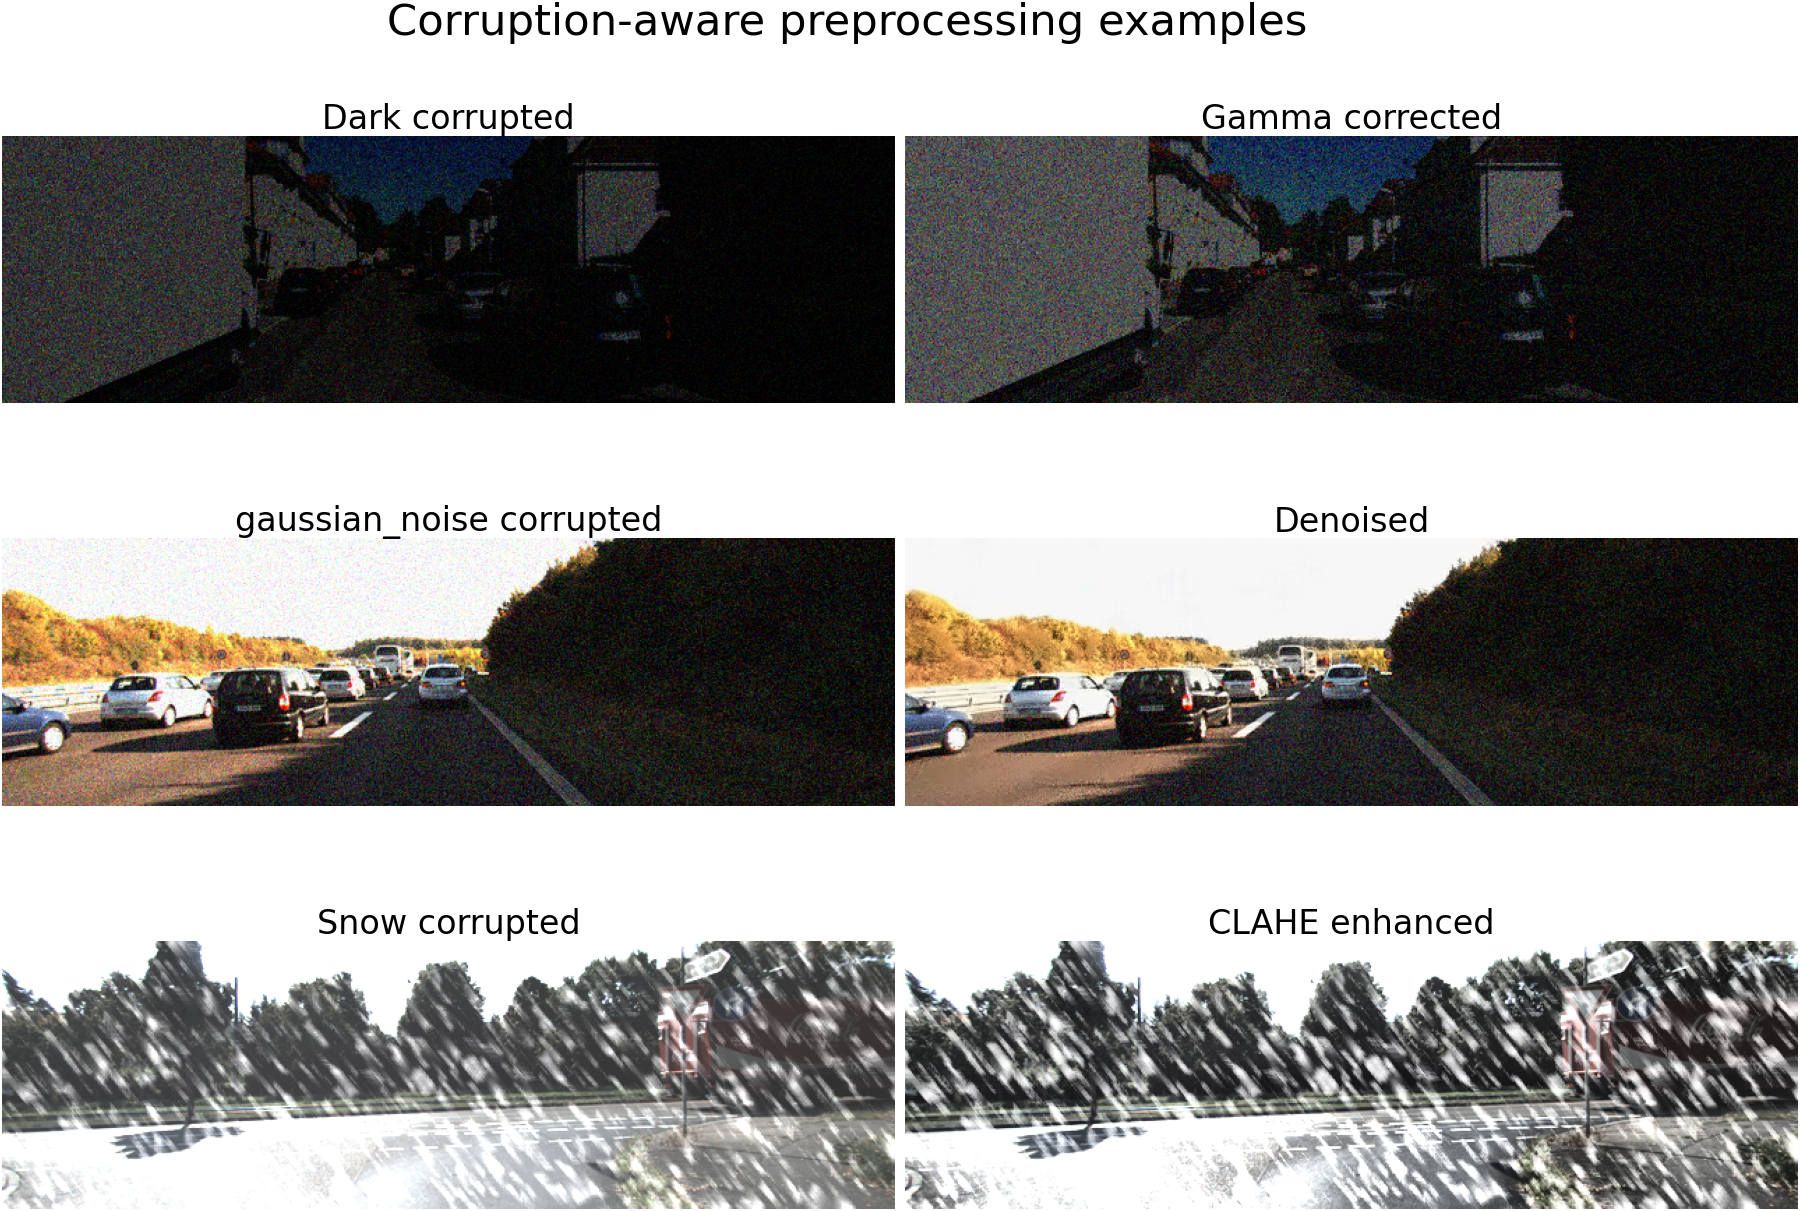
\includegraphics[width=0.78\linewidth]{figures/preprocessing_examples_3x2_recommended.png}
\caption{Preprocessing examples used in the auto-conservative strategy. Row 1 shows gamma correction for dark corruption, Row 2 shows denoising for noise corruption, and Row 3 shows CLAHE for snow corruption.}
\label{fig:preprocessing-pairs}
\end{figure}

% ============================================================
\section{Results}
% ============================================================

\subsection{Experimental Setup}

The results section follows the same logic as the project: first we report the break-it analysis, then we report the improve-it experiments. No model training or fine-tuning is performed. All methods use the pretrained MiDaS DPT-Hybrid-384 model.

For the break-it stage, we evaluate MiDaS on NYU Depth V2, DIODE, and KITTI-C. NYU Depth V2 serves as a clean indoor baseline. DIODE tests domain shift between indoor and outdoor scenes. KITTI-C tests visual corruption robustness.

For the improve-it stage, we focus on KITTI-C because it provides explicit corruption labels and severity levels. The KITTI-C manifest contains 63,427 image rows, among which 59,332 images have valid KITTI ground-truth depth and are used for evaluation.

We compare three settings:
\begin{itemize}[leftmargin=*]
    \item \textbf{Baseline}: corrupted KITTI-C image directly passed into MiDaS.
    \item \textbf{Naive Auto}: corruption-aware preprocessing using gamma correction, CLAHE, and denoising.
    \item \textbf{Auto-Conservative}: a refined preprocessing policy that only applies transformations to corruption types where preprocessing empirically improved performance.
\end{itemize}

\subsection{Break-It Results Across Datasets}

\begin{table}[H]
\centering
\begin{tabular}{lccc}
\toprule
Dataset / Split & AbsRel & RMSE & $\delta_1$ \\
\midrule
NYU Depth V2 & 0.1450 & 0.4880 & 0.8192 \\
DIODE overall & 0.3836 & 4.3382 & 0.6607 \\
DIODE indoor & 0.1499 & -- & 0.8181 \\
DIODE outdoor & 0.5540 & -- & 0.5460 \\
\bottomrule
\end{tabular}
\caption{Break-it evaluation across clean indoor and domain-shift datasets. MiDaS performs strongly on clean indoor data but degrades substantially on outdoor DIODE scenes.}
\label{tab:cross-dataset-breakit}
\end{table}

The cross-dataset results show a clear domain gap. MiDaS performs well on NYU Depth V2 and DIODE indoor scenes, where indoor layouts and depth ranges are relatively structured. However, DIODE outdoor scenes are substantially harder, with AbsRel increasing to 0.5540 and $\delta_1$ dropping to 0.5460. This supports the first break-it conclusion: even a robust pretrained model remains sensitive to domain shift.

\subsection{KITTI-C Break-It Analysis}

On KITTI-C, the baseline MiDaS model shows consistent degradation under visual corruptions. The clean setting has AbsRel approximately 0.301 and $\delta_1$ approximately 0.511. Under stronger corruptions, performance becomes worse; at severity 5, AbsRel rises to approximately 0.351 and $\delta_1$ drops to approximately 0.451.

\begin{table}[H]
\centering
\begin{tabular}{lcc}
\toprule
KITTI-C setting & AbsRel & $\delta_1$ \\
\midrule
Clean & 0.301 & 0.511 \\
Severity 5 average & 0.351 & 0.451 \\
\bottomrule
\end{tabular}
\caption{Break-it summary for KITTI-C. Higher corruption severity leads to worse MiDaS performance.}
\label{tab:kittic-severity-breakit}
\end{table}

Among corruption types, snow produces the largest degradation relative to the clean setting. The baseline clean AbsRel is 0.3006, while snow reaches 0.4233. This corresponds to an approximate 40.8\% relative increase in AbsRel:
\[
\frac{0.4233 - 0.3006}{0.3006} \times 100\% \approx 40.8\%.
\]
Structural corruptions such as blur and frost also have strong negative effects, while some illumination or quantization changes are less damaging. These observations motivated the improve-it stage: if certain corruptions damage specific visual cues, targeted preprocessing may partially restore those cues before MiDaS inference.

\subsection{Overall Quantitative Results}

\begin{table}[H]
\centering
\begin{tabular}{lccc}
\toprule
Metric & Baseline & Naive Auto & Auto-Conservative \\
\midrule
AbsRel & 0.330317 & 0.330889 & \textbf{0.329626} \\
SqRel & 2.414640 & 2.417065 & \textbf{2.405068} \\
RMSE & 7.039359 & 7.046996 & \textbf{7.029620} \\
RMSE$_{\log}$ & \textbf{1.179418} & 1.186824 & 1.183067 \\
$\delta_1$ & 0.472845 & 0.471136 & \textbf{0.473361} \\
$\delta_2$ & 0.763958 & 0.763413 & \textbf{0.764779} \\
$\delta_3$ & 0.881774 & 0.881666 & \textbf{0.882166} \\
\bottomrule
\end{tabular}
\caption{Overall KITTI-C results averaged over 59,332 evaluated images. Auto-conservative achieves the best performance on most metrics.}
\label{tab:overall-results}
\end{table}

The naive auto strategy slightly worsens the overall average compared with baseline. In contrast, the auto-conservative strategy improves AbsRel, SqRel, RMSE, $\delta_1$, $\delta_2$, and $\delta_3$.

\subsection{Per-Corruption Results}

\begin{table*}[t]
\centering
\scriptsize
\resizebox{\textwidth}{!}{
\begin{tabular}{lccc|ccc|ccc}
\toprule
& \multicolumn{3}{c|}{Baseline}
& \multicolumn{3}{c|}{Naive Auto}
& \multicolumn{3}{c}{Auto-Conservative} \\
Corruption & AbsRel & RMSE & $\delta_1$
& AbsRel & RMSE & $\delta_1$
& AbsRel & RMSE & $\delta_1$ \\
\midrule
brightness & 0.3019 & 6.5205 & 0.5072 & 0.3012 & 6.5228 & 0.5072 & 0.3019 & 6.5205 & 0.5072 \\
clean & 0.3006 & 6.5095 & 0.5111 & 0.3006 & 6.5095 & 0.5111 & 0.3006 & 6.5095 & 0.5111 \\
color\_quant & 0.3186 & 6.8009 & 0.4865 & 0.3186 & 6.8009 & 0.4865 & 0.3186 & 6.8009 & 0.4865 \\
contrast & 0.3075 & 6.5946 & 0.5025 & 0.3183 & 6.7583 & 0.4855 & 0.3075 & 6.5946 & 0.5025 \\
dark & 0.3289 & 6.9733 & 0.4752 & 0.3277 & 6.9817 & 0.4773 & 0.3277 & 6.9817 & 0.4773 \\
defocus\_blur & 0.3511 & 7.3216 & 0.4388 & 0.3511 & 7.3216 & 0.4388 & 0.3511 & 7.3216 & 0.4388 \\
elastic\_transform & 0.3045 & 6.5439 & 0.5024 & 0.3045 & 6.5439 & 0.5024 & 0.3045 & 6.5439 & 0.5024 \\
fog & 0.3116 & 6.6938 & 0.4999 & 0.3166 & 6.7439 & 0.4879 & 0.3116 & 6.6938 & 0.4999 \\
frost & 0.3458 & 7.3619 & 0.4501 & 0.3535 & 7.4621 & 0.4387 & 0.3458 & 7.3619 & 0.4501 \\
gaussian\_noise & 0.3302 & 7.1205 & 0.4759 & 0.3283 & 7.0924 & 0.4770 & 0.3283 & 7.0924 & 0.4770 \\
glass\_blur & 0.3414 & 7.2104 & 0.4514 & 0.3414 & 7.2104 & 0.4514 & 0.3414 & 7.2104 & 0.4514 \\
impulse\_noise & 0.3325 & 7.1818 & 0.4737 & 0.3323 & 7.1750 & 0.4726 & 0.3323 & 7.1750 & 0.4726 \\
iso\_noise & 0.3264 & 7.0795 & 0.4814 & 0.3235 & 7.0323 & 0.4852 & 0.3235 & 7.0323 & 0.4852 \\
jpeg\_compression & 0.3373 & 7.3158 & 0.4443 & 0.3373 & 7.3158 & 0.4443 & 0.3373 & 7.3158 & 0.4443 \\
motion\_blur & 0.3244 & 6.9631 & 0.4821 & 0.3244 & 6.9631 & 0.4821 & 0.3244 & 6.9631 & 0.4821 \\
pixelate & 0.3098 & 6.6528 & 0.4925 & 0.3098 & 6.6528 & 0.4925 & 0.3098 & 6.6528 & 0.4925 \\
shot\_noise & 0.3228 & 7.0272 & 0.4873 & 0.3218 & 7.0062 & 0.4870 & 0.3218 & 7.0062 & 0.4870 \\
snow & 0.4233 & 8.4341 & 0.3669 & 0.4180 & 8.3515 & 0.3707 & 0.4180 & 8.3515 & 0.3707 \\
zoom\_blur & 0.3337 & 7.0188 & 0.4852 & 0.3337 & 7.0188 & 0.4852 & 0.3337 & 7.0188 & 0.4852 \\
\bottomrule
\end{tabular}
}
\caption{Per-corruption KITTI-C results. Auto-conservative preserves baseline performance on corruptions where naive preprocessing was harmful, while retaining gains on dark, snow, and noise corruptions.}
\label{tab:per-corruption-results}
\end{table*}

\subsection{Naive Auto Policy Analysis}

The naive auto policy improves some corruption types, especially snow and noise corruptions, but hurts others. Compared with baseline, naive auto improves:
\begin{itemize}[leftmargin=*]
    \item \texttt{snow}: 0.4233 $\rightarrow$ 0.4180 AbsRel
    \item \texttt{gaussian\_noise}: 0.3302 $\rightarrow$ 0.3283 AbsRel
    \item \texttt{iso\_noise}: 0.3264 $\rightarrow$ 0.3235 AbsRel
    \item \texttt{shot\_noise}: 0.3228 $\rightarrow$ 0.3218 AbsRel
    \item \texttt{dark}: 0.3289 $\rightarrow$ 0.3277 AbsRel
\end{itemize}

However, it significantly degrades:
\begin{itemize}[leftmargin=*]
    \item \texttt{contrast}: 0.3075 $\rightarrow$ 0.3183 AbsRel
    \item \texttt{fog}: 0.3116 $\rightarrow$ 0.3166 AbsRel
    \item \texttt{frost}: 0.3458 $\rightarrow$ 0.3535 AbsRel
\end{itemize}

This suggests that CLAHE can amplify artifacts or distort image statistics in fog, frost, and contrast corruptions.

\subsection{Auto-Conservative Policy Analysis}

Based on the failure modes of the naive auto policy, we designed an auto-conservative policy. This policy applies gamma correction for \texttt{dark}, CLAHE for \texttt{snow}, denoising for noise corruptions, and no preprocessing for all other corruptions. This avoids the degradation observed on \texttt{contrast}, \texttt{fog}, and \texttt{frost}.

As a result:
\[
\mathrm{AbsRel}: 0.330317 \rightarrow 0.329626,
\]
\[
\mathrm{RMSE}: 7.039359 \rightarrow 7.029620,
\]
\[
\delta_1: 0.472845 \rightarrow 0.473361.
\]
Although the gains are modest, they are meaningful because the method does not retrain or modify MiDaS.

\subsection{Qualitative Results}

\begin{figure}[H]
\centering
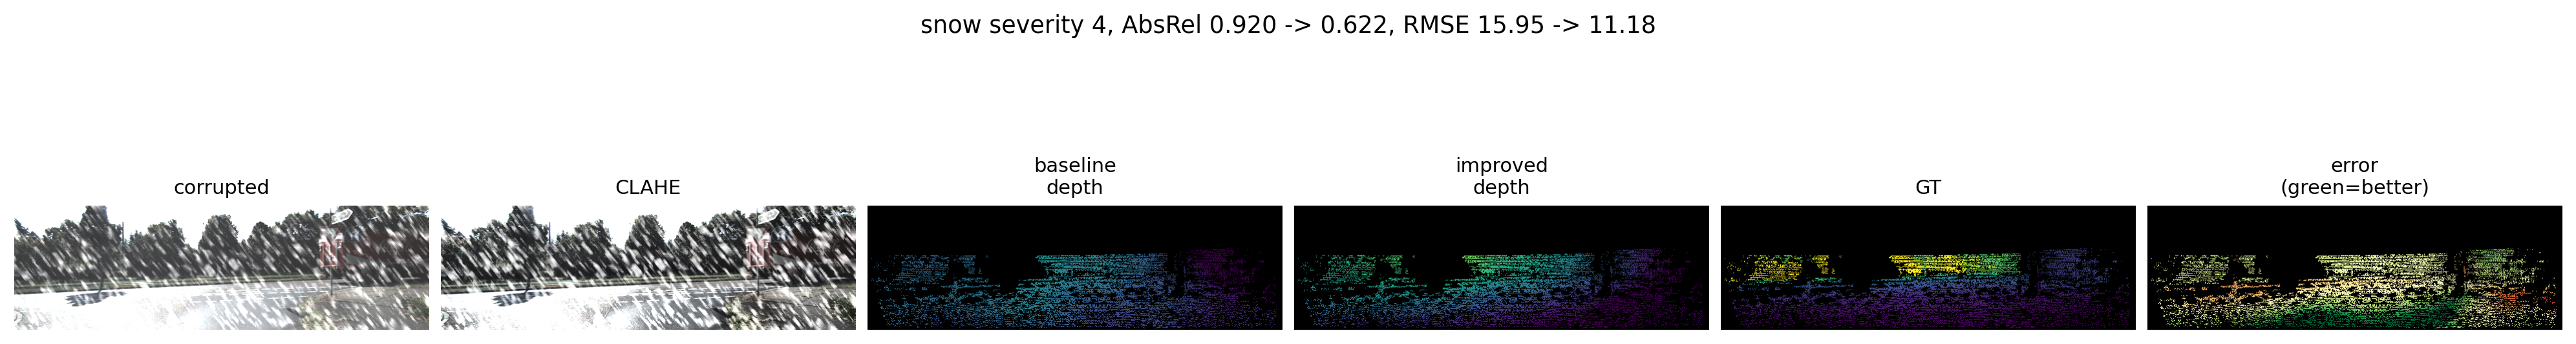
\includegraphics[width=\linewidth]{figures/figure1_snow_corruption.png}
\caption{Snow corruption example. Columns show corrupted input, CLAHE result, baseline depth, improved depth, KITTI ground truth, and error reduction map. Green in the error map indicates lower relative error after preprocessing.}
\label{fig:snow-qualitative}
\end{figure}

\begin{figure}[H]
\centering
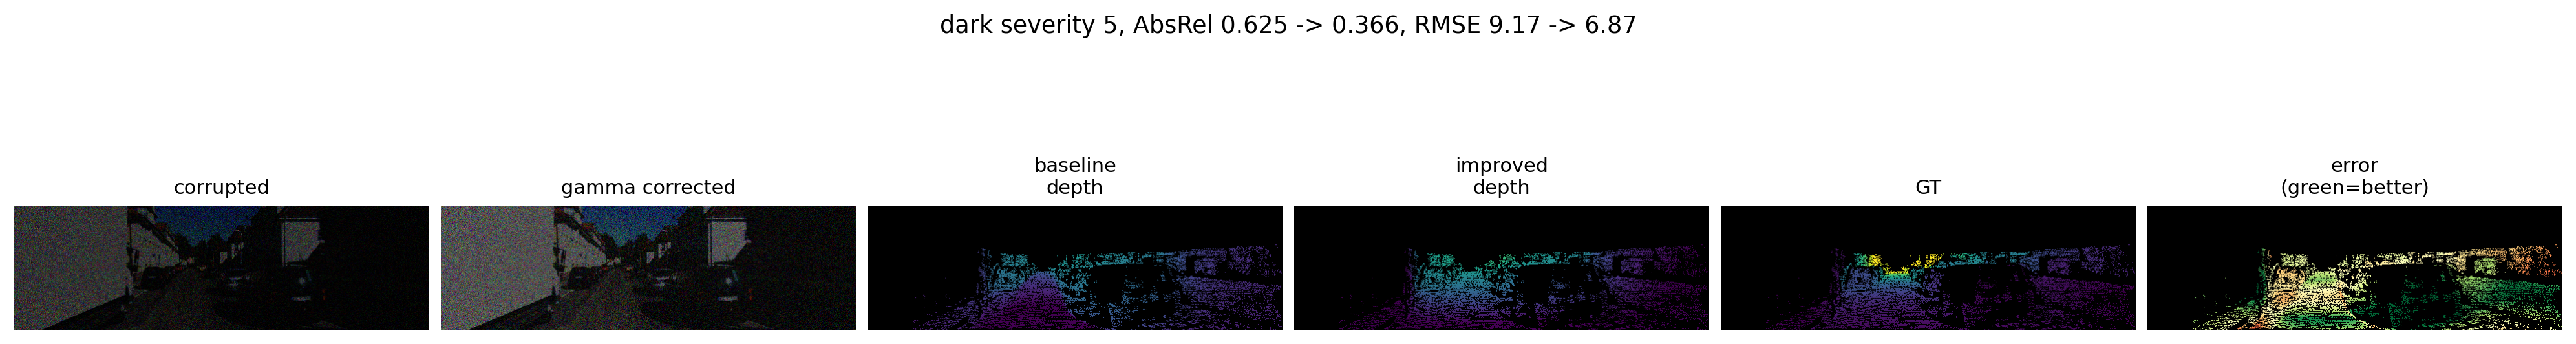
\includegraphics[width=\linewidth]{figures/figure2_dark_corruption.png}
\caption{Dark corruption example. Columns show corrupted input, gamma-corrected input, baseline depth, improved depth, KITTI ground truth, and error reduction map. Gamma correction brightens low-light regions before MiDaS inference.}
\label{fig:dark-qualitative}
\end{figure}

\begin{figure}[H]
\centering
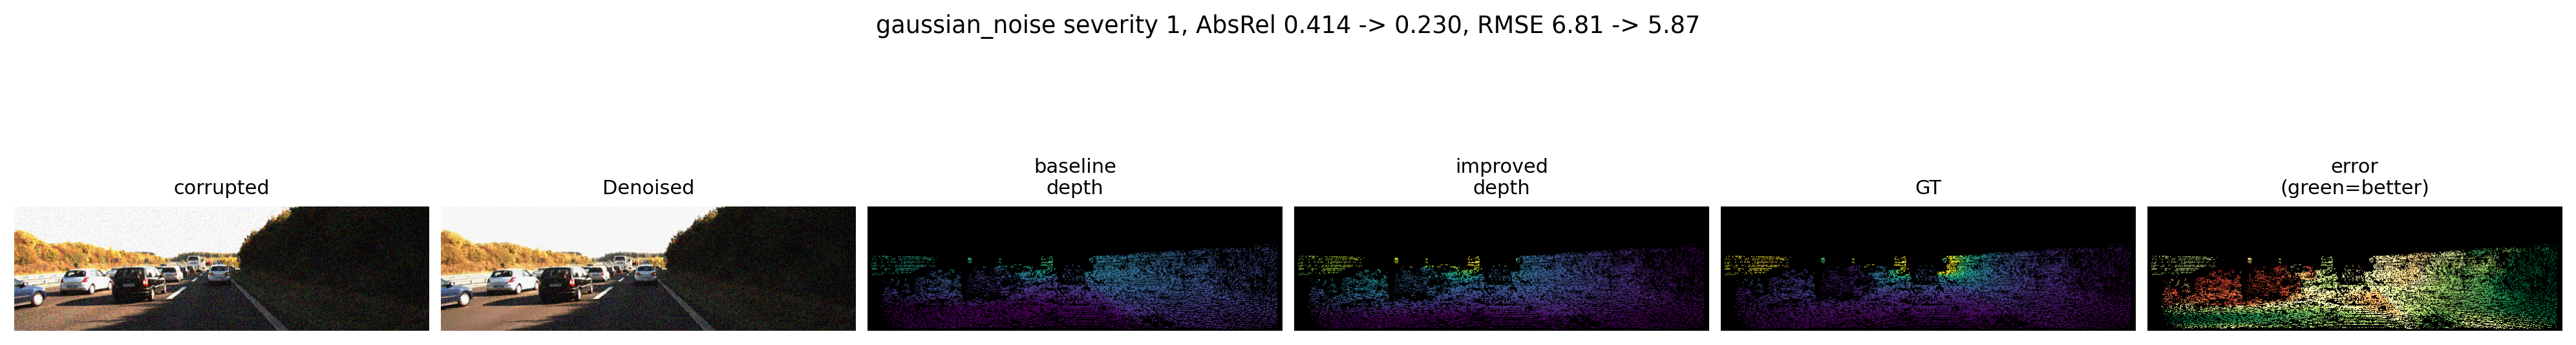
\includegraphics[width=\linewidth]{figures/figure3_noise_corruption.png}
\caption{Noise corruption example. Columns show corrupted input, denoised input, baseline depth, improved depth, KITTI ground truth, and error reduction map. Denoising suppresses high-frequency sensor noise before MiDaS inference.}
\label{fig:noise-qualitative}
\end{figure}

Qualitative examples show that snow weakens road boundaries and object edges, dark corruption suppresses useful low-light structure, and noise corruptions produce distributed local errors across textured regions. The conservative preprocessing strategy reduces some of these local failures without modifying corruption types where preprocessing is harmful.

% ============================================================
\section{Discussion and Conclusions}
% ============================================================

\subsection{Discussion of Results}

The break-it results show that MiDaS is not equally robust across all evaluation settings. It performs strongly on clean indoor benchmarks such as NYU Depth V2 and DIODE indoor, but degrades on DIODE outdoor scenes. This indicates that domain shift remains challenging even for a model trained for cross-dataset generalization. KITTI-C further shows that visual corruptions degrade performance in a structured way: stronger severity levels reduce accuracy, and snow produces the largest relative AbsRel increase compared with the clean setting.

The improve-it results show that simple image preprocessing can improve MiDaS robustness, but only when the preprocessing matches the corruption type.

Denoising improves performance on noise corruptions because it removes high-frequency image noise that can disturb depth prediction. Gamma correction slightly improves dark images by revealing low-light structure. CLAHE improves snow corruption by enhancing local contrast and restoring some edge visibility.

However, preprocessing is not universally beneficial. Applying CLAHE to fog, frost, and contrast corruptions degrades performance. These corruptions alter image appearance in ways that CLAHE may amplify incorrectly.

The auto-conservative strategy addresses this issue by only applying transformations to corruption types where we observed empirical gains. This connects the two project stages: the break-it analysis identifies which corruptions are harmful and why, while the improve-it stage tests targeted interventions for those failure modes.

\subsection{Main Insights}

Our experiments support four main insights. First, MiDaS performs well on clean indoor data but is sensitive to outdoor domain shift. Second, MiDaS is sensitive to visual corruptions in outdoor driving scenes, especially snow and severe structural corruptions. Third, preprocessing is corruption-dependent: a method that helps one corruption type may hurt another. Fourth, conservative preprocessing is more effective than broad preprocessing.

\subsection{Limitations}

Our project has several limitations. First, MiDaS predicts relative depth rather than metric depth, so scale-shift alignment is required. Although this makes evaluation possible, it can introduce variability in the reported metrics. Second, KITTI ground-truth depth is sparse, making results sensitive to valid-pixel masking and scene distribution. Third, our preprocessing policies use known corruption labels; in real deployment, the corruption type may not be known. Fourth, the improvements are modest because we do not retrain or fine-tune MiDaS. Finally, although we use NYU Depth V2 and DIODE for break-it analysis, the improve-it experiments are focused on KITTI-C; applying similar strategies to indoor and general-domain datasets remains future work.

\subsection{Future Work}

Future work could explore learned corruption detection, corruption-aware fine-tuning, test-time adaptation, video-based temporal stabilization, and stronger restoration methods. A natural next step is to replace oracle corruption labels with an automatic corruption classifier so that the conservative preprocessing policy can be used in real deployments. Another direction is to extend the improve-it stage to DIODE and NYU Depth V2 to test whether preprocessing improves domain-shift robustness beyond KITTI-C.

\subsection{Conclusion}

In this project, we evaluated the robustness of MiDaS monocular depth estimation under domain shift and visual corruptions. The break-it stage showed that MiDaS performs well on clean indoor data but degrades on outdoor domain shift and corrupted KITTI-C images. The improve-it stage showed that the naive auto preprocessing policy did not improve KITTI-C performance because CLAHE degraded fog, frost, and contrast corruptions. After analyzing this failure mode, we introduced an auto-conservative policy that applies gamma correction only to dark images, CLAHE only to snow, and denoising only to noise corruptions. The main conclusion is that robustness improvement is not only about applying stronger preprocessing, but also about deciding when not to modify the input.

% ============================================================
\section{Statement of Individual Contribution}
% ============================================================

\begin{itemize}[leftmargin=*]
    \item \textbf{Xinyin Liang}: Implemented the MiDaS inference pipeline and GPU support.
    \item \textbf{Yihui Chen}: Worked on NYU Depth V2 processing, metric evaluation, and indoor baseline failure analysis.
    \item \textbf{Kaiyu Liu}: Worked on KITTI-C corruption evaluation, preprocessing experiments, and result comparison.
    \item \textbf{Yuyang Zeng}: Worked on DIODE processing, indoor/outdoor domain-shift analysis, visualization, and report organization.
\end{itemize}

All group members contributed to project discussion, experimental design, and report writing.

% ============================================================
\section{References}
% ============================================================

\begin{enumerate}[leftmargin=*]

\item R. Ranftl, K. Lasinger, K. Hafner, K. Schindler, and V. Koltun.
``Towards Robust Monocular Depth Estimation: Mixing Datasets for Zero-shot Cross-dataset Transfer.''
IEEE Transactions on Pattern Analysis and Machine Intelligence, 2022.

\item L. Kong et al.
``RoboDepth: Robust Out-of-Distribution Depth Estimation under Corruptions.''
arXiv:2310.15171, 2023.

\item N. Silberman, D. Hoiem, P. Kohli, and R. Fergus.
``Indoor Segmentation and Support Inference from RGBD Images.''
European Conference on Computer Vision, 2012.

\item I. Vasiljevic et al.
``DIODE: A Dense Indoor and Outdoor Depth Dataset.''
arXiv:1908.00463, 2019.

\item Intel ISL.
``MiDaS.'' GitHub repository.
\url{https://github.com/isl-org/MiDaS}

\item KITTI Vision Benchmark Suite.
\url{https://www.cvlibs.net/datasets/kitti/}

\item NYU Depth V2 Dataset.
\url{https://cs.nyu.edu/~fergus/datasets/nyu_depth_v2.html}

\item DIODE Dataset.
\url{https://diode-dataset.org}

\item RoboDepth Benchmark.
\url{https://github.com/ldkong1205/RoboDepth}

\item OpenCV Documentation.
\url{https://docs.opencv.org/}

\end{enumerate}

\end{document}
